\pagebreak
\subsection{Time Constant and Gain} %\label{put a label here and uncomment}
\textbf{Name: Group 510}\\
\textbf{Date: 30/09 - 2015}

\subsubsection{Purpose}
The purpose of this test is to find the motors time constant $\tau$ and gain. This is done by measuring the motors step response.

\subsubsection{Setup}
\begin{figure}[H]
  \centering
	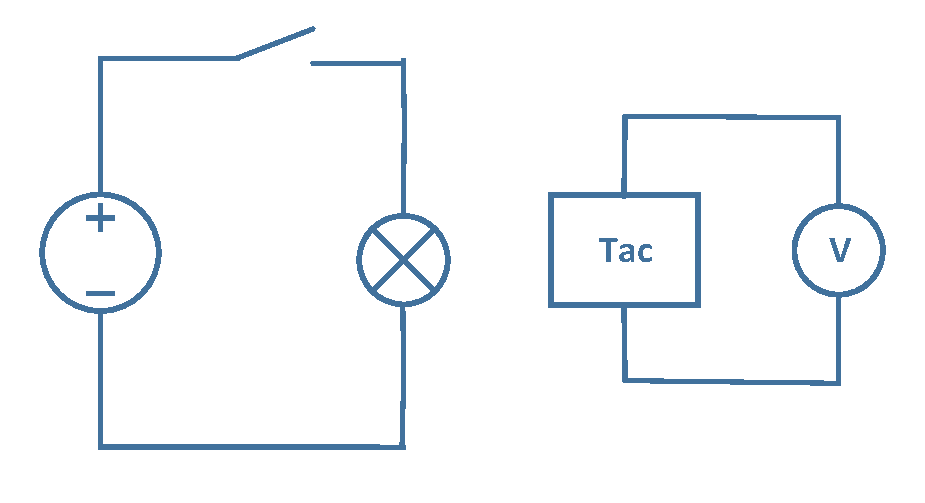
\includegraphics[scale=0.5]{figures/MotorTest8.pdf}
	\caption{A diagram of the test setup}
\end{figure}

\subsubsection{List of Equipment}

\begin{table}[H]
\begin{tabular}{|l|l|p{4cm}|}
\hline%------------------------------------------------------------------------------------
  \textbf{Instrument}                        &  \textbf{AAU-no.}  &  \textbf{Type}       \\
\hline%------------------------------------------------------------------------------------
  Oscilloscope                               &  64672             &  Agilent DSO6034A    \\
\hline%------------------------------------------------------------------------------------
  Power Supply ($0 - 32$ V) ($0 - 10$ A)     &  77076             &  Ea - ps 7032 - 100  \\
\hline%------------------------------------------------------------------------------------
  Optical tachometer                         &  77087             &  Compact             \\
\hline%------------------------------------------------------------------------------------
\end{tabular}
\end{table}

\subsubsection{Procedure}

\begin{enumerate}
  \item Turn on the oscilloscope, and connect one channel to the power supply, and another to the tachometer.
  \item On the oscilloscope press the "trigger mode"-key choose the "normal"-option, set the trigger to "rising-edge", and the trigger source to the channel connected to the power supply.
  \item To prevent false triggering on the oscilloscope set the trigger value to \num{4,50}V with the turn-key.
  \item Press "single"-key on oscilloscope.
  \item Turn on the power supply at 5 volt.
  \item Insert a USB-flash drive in the oscilloscope and press the save key to extract the data.
\end{enumerate}

\subsubsection{Results}

\begin{figure}[H]
  \centering
 	%Trim margins @:   left        bottom       right       top
 	\adjustbox{ trim = {.15\width} {.30\height} {.15\width} {.30\height}, clip }
  {
    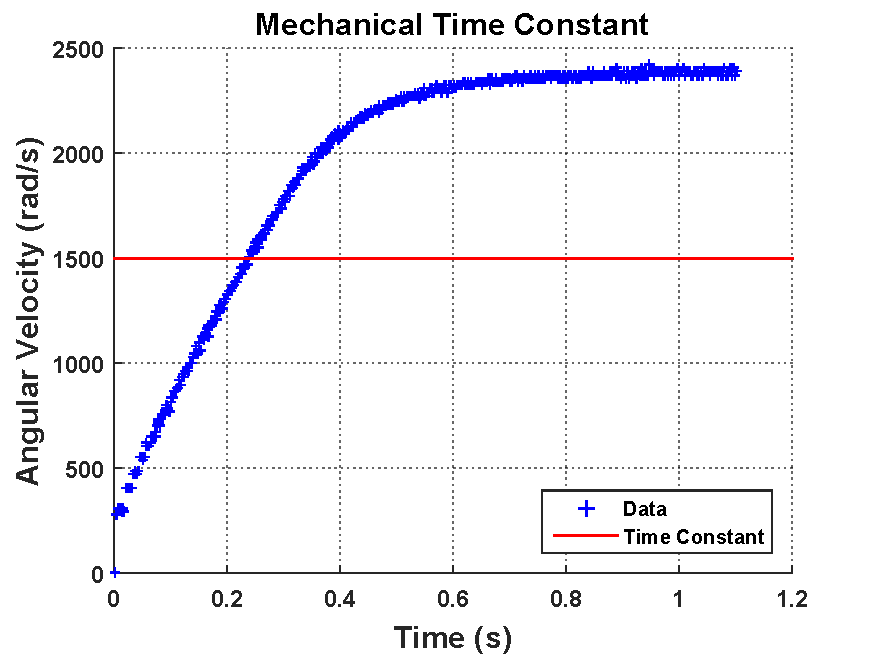
\includegraphics[width=.8\textwidth]{figures/mechanicalTimeConstant.pdf}
  }
	\caption{Plot of the mechanical time constant results}
	\label{mechanicalTimeConstant}
\end{figure}

The graph in \figref{mechanicalTimeConstant} shows the angular velocity of the motor over time. The read line shows the time constant at \si{\num{63.2} \%} of max angular velocity. In the data the mechanical time constant is found to be:
%
\begin{align}
  \eq{\tau_{mec}}{\num{0.238}} \unit{s}\nonumber
\end{align}

\begin{figure}[H]
  \centering
 	%Trim margins @:   left        bottom       right       top
 	\adjustbox{ trim = {.15\width} {.30\height} {.15\width} {.30\height}, clip }
  {
    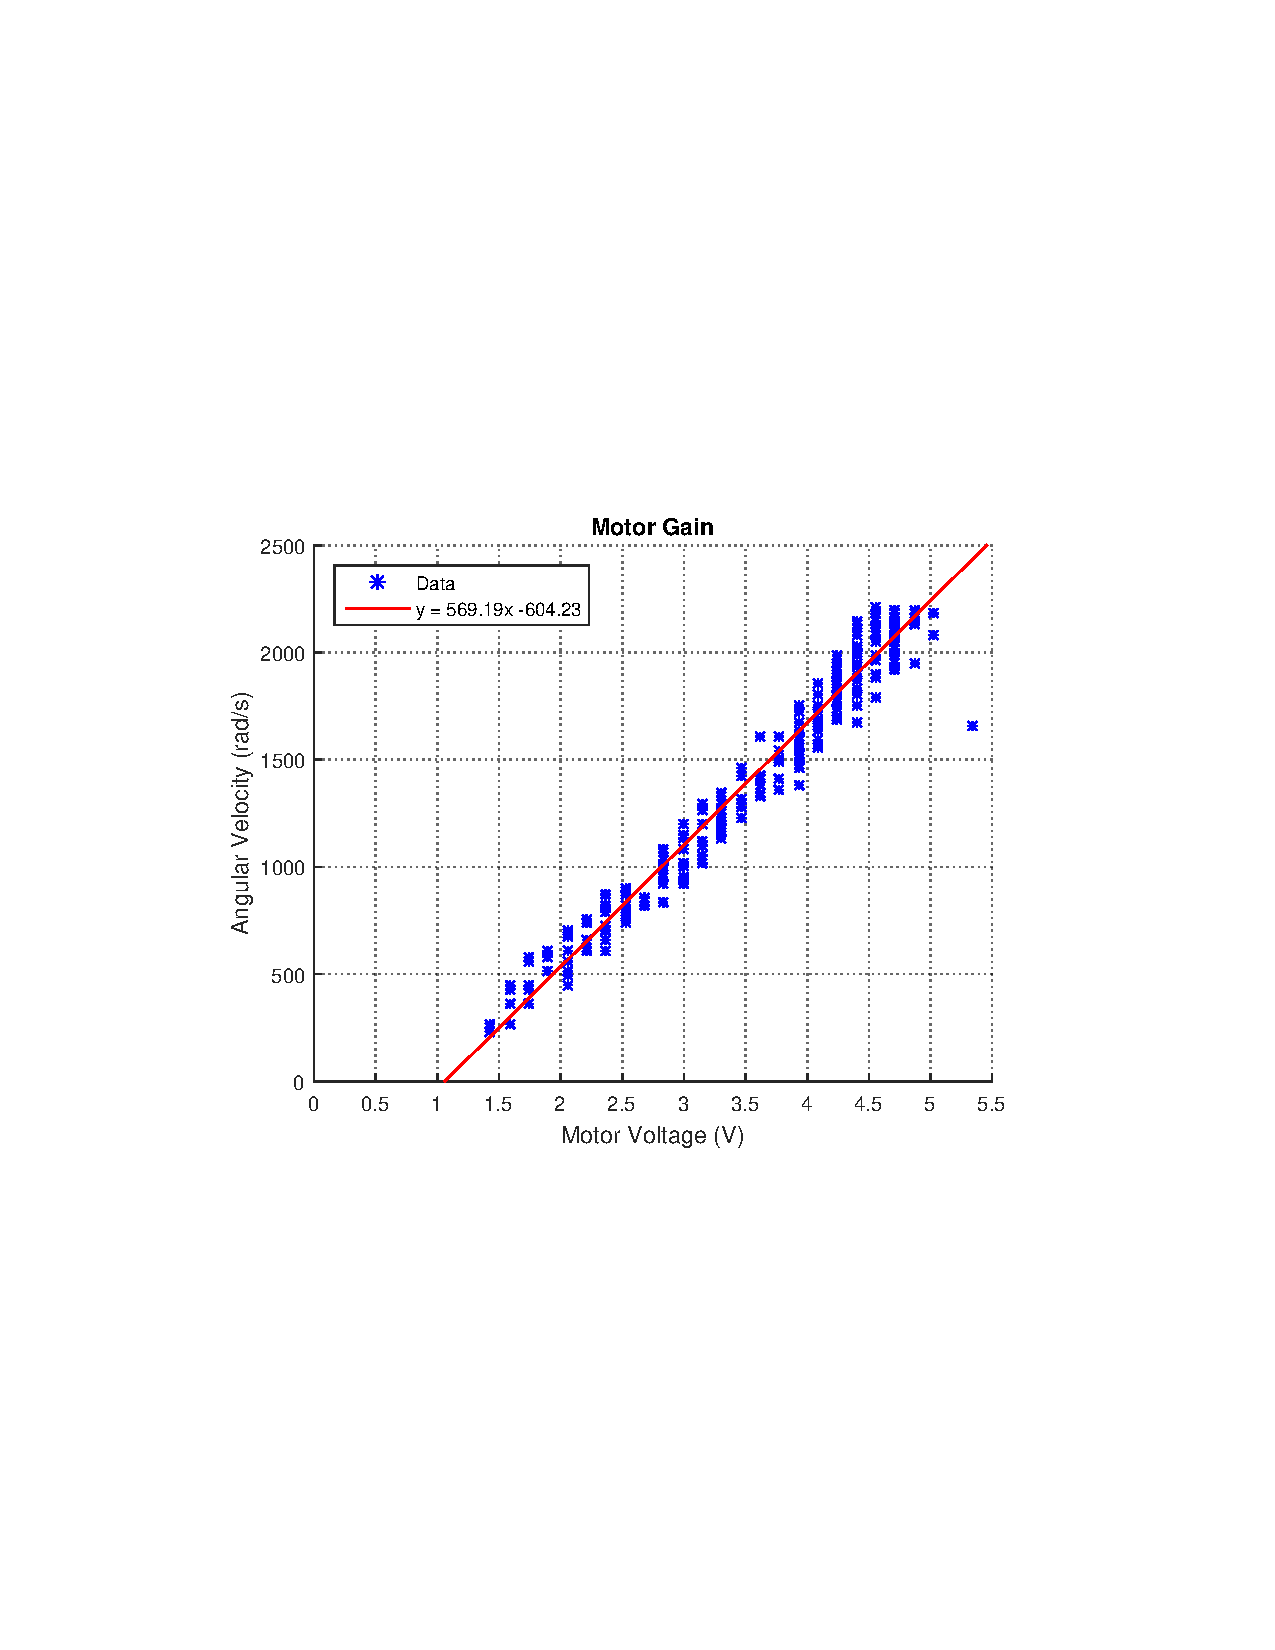
\includegraphics[width=.8\textwidth]{figures/motorGain.pdf}
  }
	\caption{Plot of the motor gain results}
	\label{motorGain}
\end{figure}

The graph in \figref{motorGain} shows motor voltage in relation to the angular velocity, which reveals the gain, \si{K} of the system, as the slope of the least square regression line:
%
\begin{align}
  \eq{K}{\num{569.19}} \unit{\cdot}\nonumber
\end{align}
